\clearpage

\setcounter{page}{1}
\setcounter{section}{0}
\counterwithin{figure}{section} % add section number to table
\counterwithin{table}{section}
\renewcommand{\thesection}{\Alph{section}} % numbering to letters
\maketitlesupplementary
\begin{abstract}
    We provide additional details in the following:
\begin{enumerate}
    \item A website including additional video results (\cref{supp:website}).
    \item Implementation details of \ours, including more training details and model architecture (\cref{supp:implementation}).
    \item Additional details on training data generation (\cref{supp:training_data}).
    \item Finetuning strategies (GA vs DiT) (\cref{supp:finetuning}).
    \item Multi-modal encoding using RGB Video VAE (\cref{supp:vae_encoding}).
    \item Analysis of different 3DGS artifacts
    (\cref{supp:3dgs_artifact}).
    \item Comparison of refinement and direction Generation
    (\cref{supp:refinement_vs_generation}).
    \item Additional qualitative results (\cref{supp:add_results}).
    \item Limitations and future work (\cref{supp:limitations}).
\end{enumerate}
\end{abstract}

% \section{Additional Results}
\section{Website and Video}
\label{supp:website}
We provide additional video results in the \href{http://research.zhuliyuan.net/projects/GaussFusion/}{project page} to comprehensively demonstrate the performance of GaussFusion. The website includes (1) multi-modal GP-buffer visualizations displaying the geometry-aware representations (alpha, color, depth, normal, and inverse covariance maps) that inform our video generation process; (2) novel-view refinement results with side-by-side comparisons against baseline methods; and (3) refinement results on feed-forward reconstructions from DepthSplat~\cite{xu2024depthsplat} with side-by-side comparisons against baselines.


\section{Additional Implementation Details}
\label{supp:implementation}
\paragraph{Architecture Details.}
Our flow transformer follows the Wan DiT~\cite{wan2025} backbone with 30 DiT blocks (hidden dimension 1536) and a final DiT head, as illustrated in Fig.~\ref{fig:architecture}. On top of this backbone we interleave lightweight Geometry Adapter (GA) blocks: after every two DiT blocks we insert one GA block, resulting in 15 GA blocks in total~\cite{vace_wan}. Each GA block operates at the same dimensionality as the DiT backbone and follows the structure shown in Fig.~\ref{fig:architecture}, consisting of LayerNorm, self-attention, cross-attention, and an MLP. The 3DGS GP-buffer (alphas, color, depth, normals, and uncertainty) is encoded by a VAE into compact geometry tokens $\mathbf{z}_{\mathrm{g}}$ which are passed to a 3D convolutional layer, then linearly projected to the DiT hidden size, and used as key/value in the GA attention layer. The GA produces a geometry-aware feature $\mathbf{x}_{\mathrm{g}}$, which is projected back and injected into the DiT stream via a gated residual connection, allowing geometry-conditioned features to modulate the video latents while preserving the original Wan DiT parameters.


\paragraph{Training.} We implement our code using PyTorch 2.7.1 with CUDA 12.6 on 8 NVIDIA H200 GPUs. We employ BF16 precision, FlashAttention-2~\cite{dao2023flashattention}, and ZeRO-2 sharding~\cite{aminabadi2022deepspeed} to improve training and memory efficiency. We set batchsize per GPU to 1 and apply gradient accumulation every 4 steps to have an effective batchsize of 32. The training videos have a spatial resolution of 480$\times$832 and 81 frames. We use Wan2.1~\cite{wan2025} VAE to precompute the video latents of all the training pairs for efficiency. The video latents have a spatial resolution of 60$\times$104 and 21 frames in latent space.


\begin{figure}[h]
    \centering
    \includegraphics[width=\linewidth]{fig/image/training_curve.pdf}
    \caption{\textbf{Training Curve Comparison Between DiT and GA.} We visualize the training loss (left) and validation PSNR (right) over 50k iterations. The proposed GA method (orange) demonstrates faster convergence and consistently lower loss compared to the Full DiT baseline (blue). Correspondingly, GA achieves higher image restoration fidelity (PSNR) on the validation set, maintaining a clear performance margin throughout same steps of training.}
    \label{fig:training_curve}
\end{figure}

\section{Training Data Generation.}
\label{supp:training_data}
We provide more details of artifact simulation in \cref{sec:data}. We derive the training data on full DL3DV~\cite{ling2024dl3dv} and first 100 training splits (10K scenes) of RE10K~\cite{re10k}. DL3DV provides COLMAP~\cite{schoenberger2016colmap} structure-from-motion (SfM) data so we directly initialize 3DGS from SfM point clouds following the standard protocol. We also adopt random 3D point cloud initialization on 50\% of the scenes in DL3DV. Since RE10K~\cite{re10k} dataset only provides camera poses and does not provide COLMAP reconstruction data, we attempted to run COLMAP ourselves but the default COLMAP reconstruction pipeline failed on most of the RE10K scenes. Therefore we initialize the 3DGS (50\%) from random 3D point initialization and dense point map (50\%) reconstructed from MapAnything~\cite{keetha2025mapanything}. This makes RE10K a harder case because the geometry initialization of the 3DGS includes geometric errors. For optimization-based 3DGS reconstruction, we randomly select training steps from 3000, 7000, and 30000 to imitate undertrained splats.
For feed-forward reconstructions, we run MVSplat~\cite{chen2024mvsplat} and DepthSplat~\cite{xu2024depthsplat} on RE10K dataset to simulate diverse reconstruction artifacts from feed-forward models. For each scene on RE10K, we only feed three evenly distributed views (first, middle, and last) as input to the model to get the sparse-view reconstruction with artifacts.

\section{Geometry Adapter vs DiT Fine-tuning}
\label{supp:finetuning}
To support our claim in the main paper that GA-based finetuning can converge faster and provide better performance than baseline methods under the same number of training steps (see \cref{tab:ablation_artifact}), we provide the training loss and validation curve of DiT-based and GA-based finetuning in \cref{fig:training_curve}. Our GA-based finetuning converges faster in the first 10K training steps and also shows better validation performance than the full DiT-based finetuning. We notice that full DiT-based finetuning can reach similar performance \wrt GA if we train longer for 2$\times$ iterations (3 days). This demonstrates our GA design is more efficient than baselines.

\section{Multi-Modal Encoding}
\label{supp:vae_encoding}
Since the original Wan~\cite{wan2025} VAE was designed to compress RGB videos and remains frozen in our training setup, we study how effective it is to encode non-RGB modalities, \ie, depth, alphas, inverse covariance, and normal maps. We measure the encode-decode reconstruction error for each modality in the GP-Buffer using mean absolute error (MAE), mean squared error (MSE), relative error (RelErr), and squared relative error (SqRel). We run this evaluation on 400 GP-Buffer videos on DL3DV renders and report the metrics in \cref{tab:vae}. We find that depth and alpha have reconstruction errors comparable to RGB, while inverse covariance maps and normal maps exhibit slightly larger errors, likely due to their different color value distributions. This can be alleviated by finetuning the VAE on new modality data following~\cite{jiang2025geo4d,szymanowicz2025bolt3d}.


\begin{table}[h]
\centering
\footnotesize
\setlength{\tabcolsep}{4pt}
\begin{tabular}{lccccc}
\toprule
\textbf{Modality} & \# Channel & \textbf{MAE}$\downarrow$ & \textbf{MSE}$\downarrow$ & \textbf{RelErr}$\downarrow$ & \textbf{SqRel}$\downarrow$ \\
\midrule
RGB  &  3 & 0.0323 & 0.00362 & 0.0199 & 0.0217 \\
Depth&  1 & 0.0253 & 0.00252 & 0.0044 & 0.0182 \\
Alpha&  1 & 0.0138 & 0.00150 & 0.0075 & 0.0053 \\
Covar.& 3 & 0.0758 & 0.01048 & 0.0147 & 0.0847 \\
Normal& 3 & 0.1890  & 0.06684 & 0.1333 & 0.3507 \\
\bottomrule
\end{tabular}
\caption{\textbf{Per-Modality VAE Reconstruction Error.} Comparison of mean absolute error (MAE), mean squared error (MSE), relative error (RelErr), and squared relative error (SqRel).}
\label{tab:vae}
\end{table}

\section{Analysis of 3DGS Artifacts.} 
\label{supp:3dgs_artifact}
Understanding degradation patterns is key to generalizable refinement. While quantitative attribution is challenging due to the stochastic nature of 3DGS optimization (e.g., densification heuristics and camera initialization), we provide our empirical findings and insights in \cref{tab:artifact_comparison}. For \textbf{optimization-based} methods, we observe that large pose drifts generate high-frequency ``floaters,'' while sparse coverage leads to ``needle-like'' over-elongated Gaussians. 
In contrast, \textbf{feed-forward} models~\cite{xu2024depthsplat,chen2024mvsplat} exhibit distinct failure modes driven by regression uncertainty: they suffer from low-frequency blur (due to mean-seeking behavior) and global geometric warping (due to inconsistent depth estimation). Crucially, we do not simulate these artifacts via synthetic filters; instead, we induce them as direct outputs of the 3DGS pipeline by modulating input conditions. This allows us to control the severity of intrinsic failures, ensuring \ours generalizes to practical real-world scenarios.

\begin{table}[h]
\centering
% Resize the table to fit the width of the column
\resizebox{\columnwidth}{!}{%
\begin{tabular}{lll}
\toprule
Feature & Optimization-Based 3DGS & Feed-Forward 3DGS \\ 
\midrule
Primary visual flaw & High-frequency noise (Floaters) & Low-frequency blur (Oversmoothing) \\
Geometry artifacts & "Needles" (over-stretched covariance) & Global depth warping / Scale ambiguity \\
Unseen areas & Empty / Holes & Plausible but blurry (learned priors) \\
Source of error & Overfitting (high variance) & Uncertainty / Regression to mean \\
\bottomrule
\end{tabular}%
}
% \vspace{-pt}
\caption{\textbf{Empirical Analysis of Artifacts in 3DGS.}}
\label{tab:artifact_comparison}
\end{table}


\section{Refinement vs. Direct Generation.} 
\label{supp:refinement_vs_generation}
We evaluate the direct generation baseline, Matrix3D~\cite{lu2025matrix3d}, on DL3DV and find \ours significantly outperforms it (PSNR 19.36 vs. 11.30; LPIPS  0.279 vs. 0.639). Direct generation methods struggle with consistency due to limited context windows and the difficulty of implicitly learning precise 3D projections. Our refinement paradigm uses the 3DGS as an explicit 3D memory. By decoupling the camera model via rasterization, we enforce mathematically correct projections, preventing the drift in pure generation. 

\section{Additional Qualitative Results}
\label{supp:add_results}
In this section, we provide example visuals on the modalities comprising the GP-Buffer input and qualitative comparisons against baseline methods. 

\paragraph{GP-Buffer Visualization.}
The GP-Buffer encodes a set of geometry-related modalities, therefore inheriting the characteristic artifacts of 3D Gaussian splatting, that serve as the \emph{input} to our method. As shown in Figure~\ref{fig:gp_buffer_vis}, it contains five modalities: \textit{color}, \textit{alpha}, \textit{depth}, \textit{normal}, and \textit{inverse covariance}. These inputs not only describe the reconstructed scene but also make visible the distortions, noise, and inconsistencies that arise from imperfect geometry or view-dependent effects in the underlying 3DGS representation.
As shown in \cref{fig:gp_buffer_vis}, the color channel reflects photometric artifacts such as blurred textures or multi-view inconsistencies. The alpha channel highlights irregular opacity and over-accumulation in regions where splats overlap or geometry is uncertain. Depth maps often expose depth bleeding and surface discontinuities, while the surface normals reveal noisy or unstable local orientations, especially near edges or thin structures. Finally, the inverse covariance map visualizes the anisotropy and uncertainty of individual Gaussians; high-variance or poorly constrained areas appear as strong patterns in this channel. Together, these complementary modalities make explicit how reconstruction artifacts manifest across the 3D representation, supporting our claim that the GP-Buffer encodes both scene geometry and its associated imperfections.


\paragraph{Additional Qualitative Comparison.}
We provide additional novel-view refinement comparison in \cref{fig:supp_image_refine}. The top three rows correspond to the results on optimization-based 3DGS reconstruction and the bottom three feed-forward model reconstruction.
Compared to methods in both categories, our method (\ours) achieves sharper textures, more consistent geometry, and superior visual refinement, closely matching the ground-truth images. \cref{fig:supp_recon} presents the qualitative comparison on refined 3DGS reconstruction. \ours excels at challenging cases where in the original reconstruction part of the geometry is missing/wrong: while baseline methods smear out the artifacts and blur out those regions, \ours can faithfully refine/repaint the geometry, demonstrating superior photorealism and cross-view consistency.

\section{Limitations and Future Work}
\label{supp:limitations}
\paragraph{Limitations.}
\ours, although better than baselines, performs less effectively on videos with rapid motion or severe motion blur, where the VAE struggles to encode clean latent representations, leading to degraded generation quality. Our model operates on a context window of 81 frames. To process longer videos, we adopt a bidirectional sliding-window strategy, where the last frame of the current prediction is used as the first frame of the next window. While this approach maintains short-term temporal consistency across a few hundred frames, it does not fully guarantee long-term coherence or synchronization between independently generated segments.

\paragraph{Future Work.}
Future extensions could explore improved distillation techniques, such as self-forcing~\cite{huang2025selfforcing} and incorporate causal modeling with a rolling KV cache, to better support streaming or real-time applications. Another promising direction is to develop mechanisms that enable the video generative model to directly update the 3D Gaussian parameters online, allowing dynamic scene refinement without post-hoc optimization.





\begin{figure*}[h]
    \centering
    % 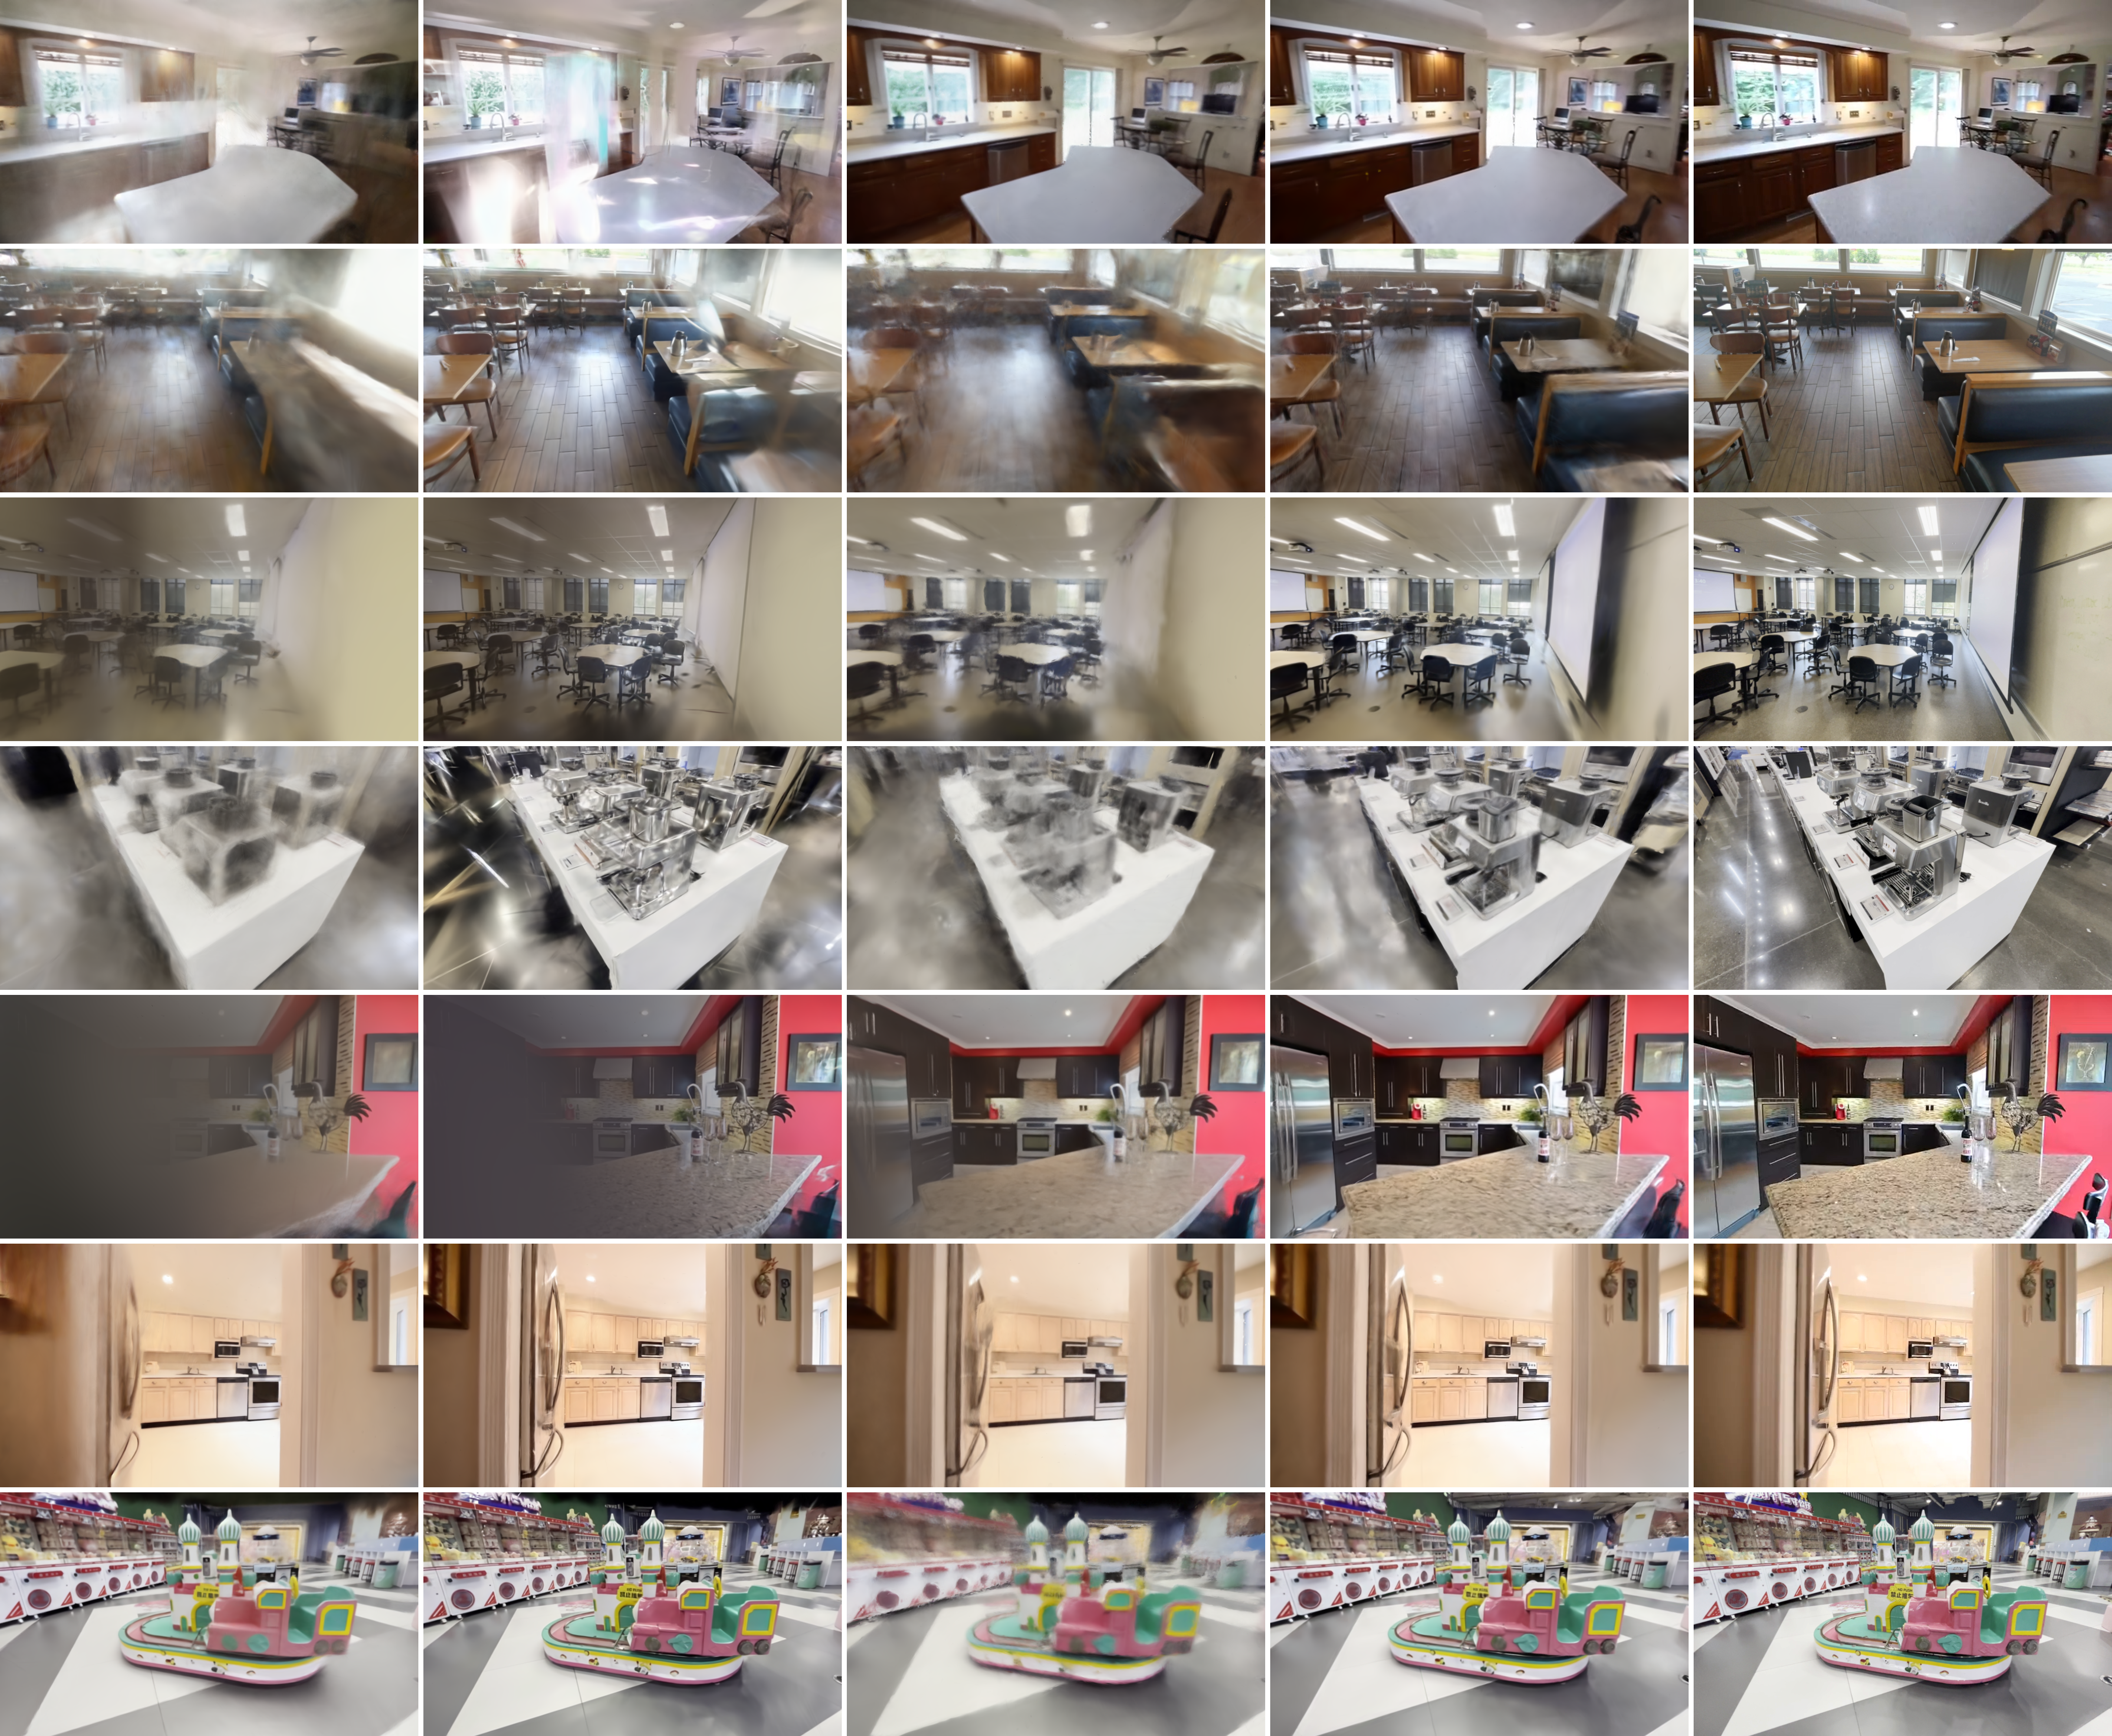
\includegraphics[width=\linewidth]{fig/image/supp_recon.png}
    \includegraphics[width=0.8\linewidth]{fig/image/gp-buffer_vis.pdf}%
\caption{\textbf{GP-Buffer Sample Visualizations on DL3DV~\cite{ling2024dl3dv}.} The five comprising modalities (color, alpha, depth, normal, and inverse covariance) are the input to our model.}
    \label{fig:gp_buffer_vis}
\end{figure*}


\begin{figure*}[t]
    \centering
 \begin{tabular}{cccccc}
   
    \multicolumn{6}{c}{%
        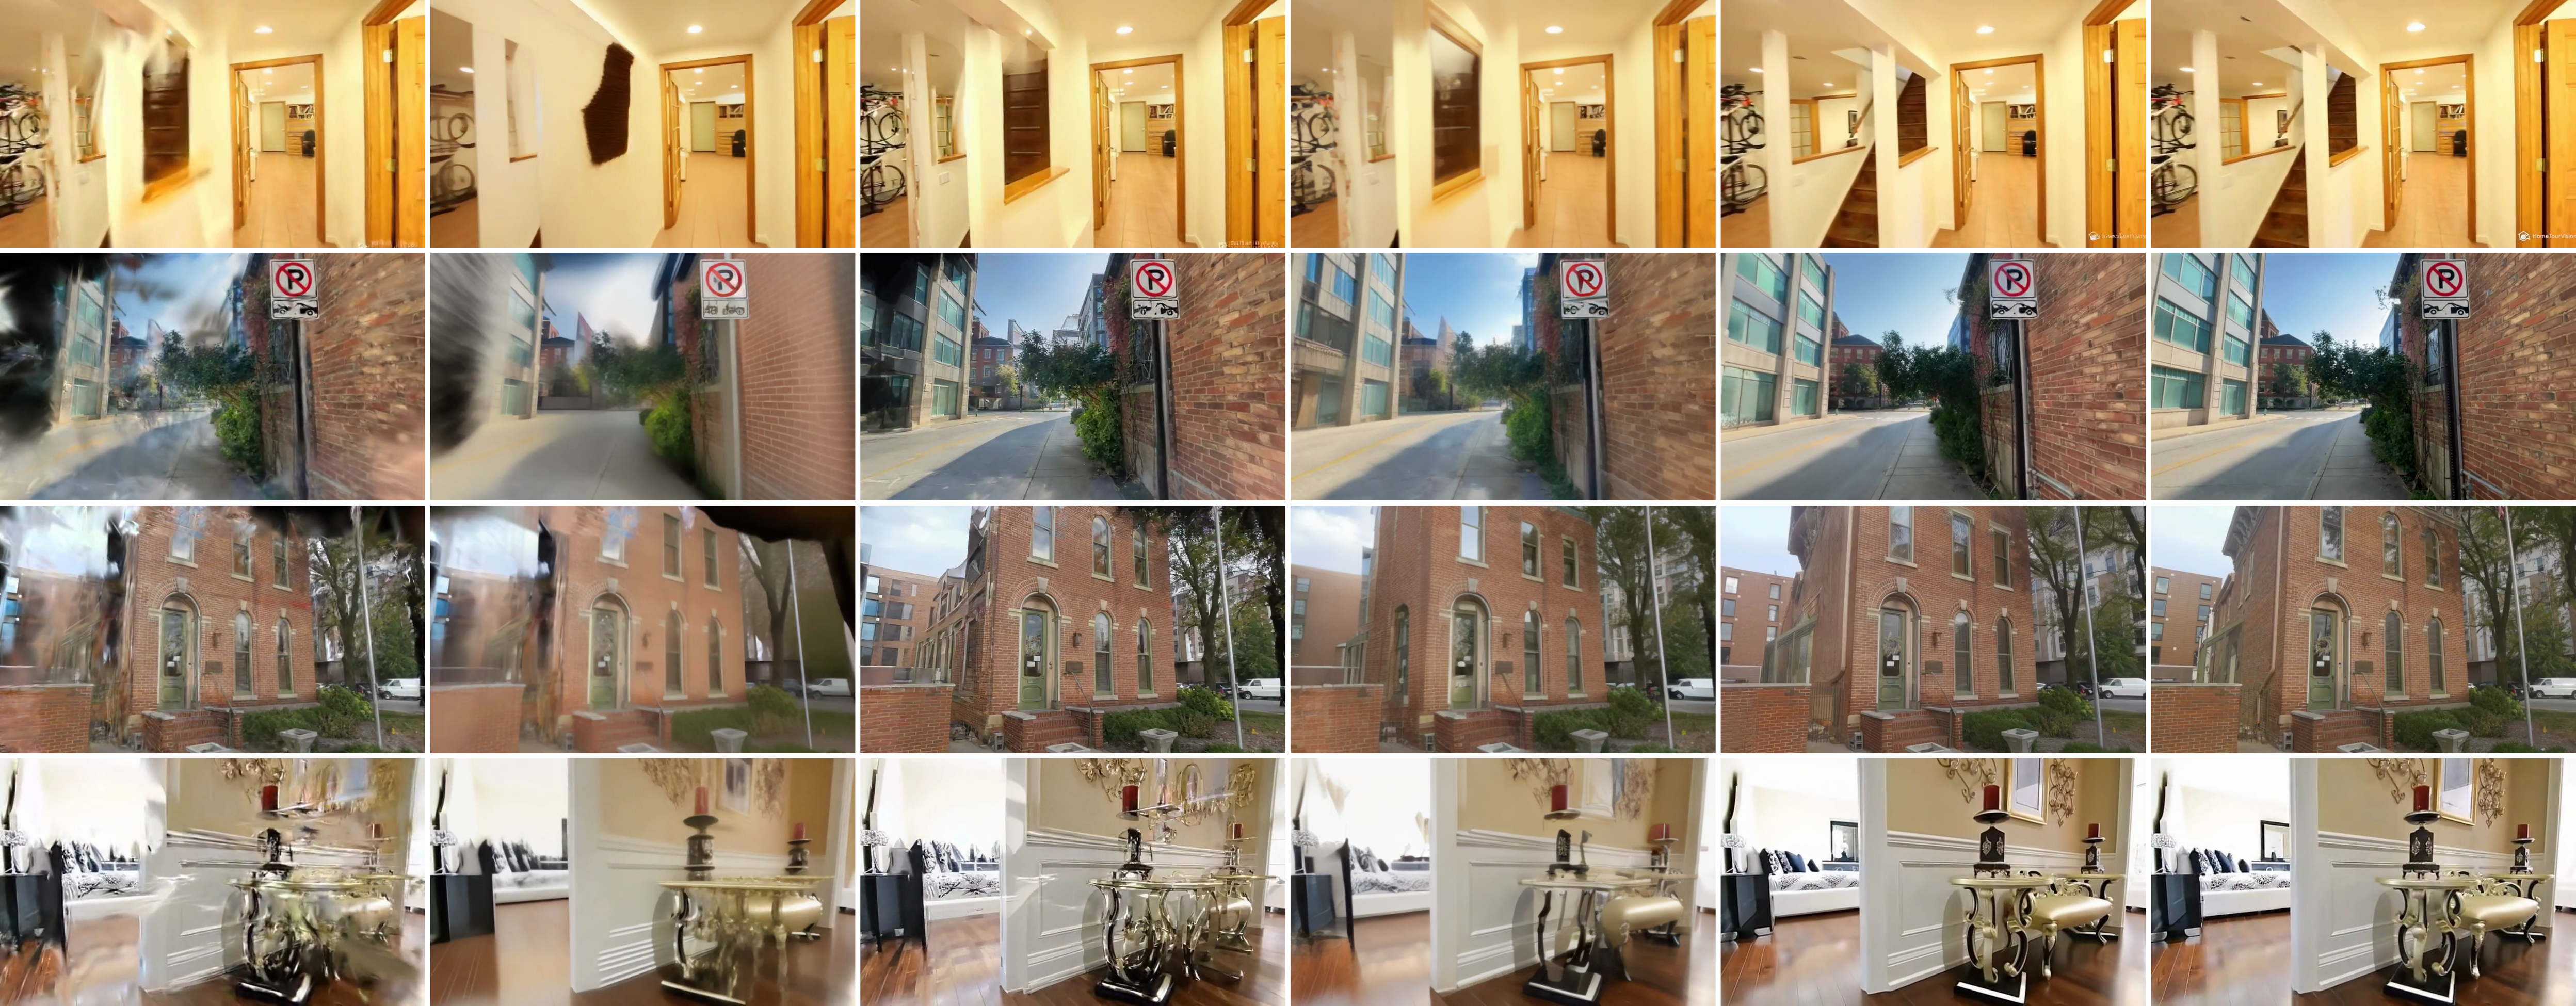
\includegraphics[width=\linewidth]{fig/image/supp_OP.png}%
    } \\
     \hspace{0.4cm} \small Splatfacto~\cite{ye2025gsplat} & 
    \hspace{0.4cm} \small GenFusion~\cite{Wu2025GenFusion} & 
    \hspace{.5cm}\small Difix3D+~\cite{wu2025difix3d} & 
    \hspace{.6cm}\small ExploreGS~\cite{Kim_2025_ExploreGS} &
    \hspace{0.2cm}\small \ours (Ours) & 
    \hspace{-0.1cm}\small Ground Truth \\
    \midrule
    \multicolumn{6}{c}{%
        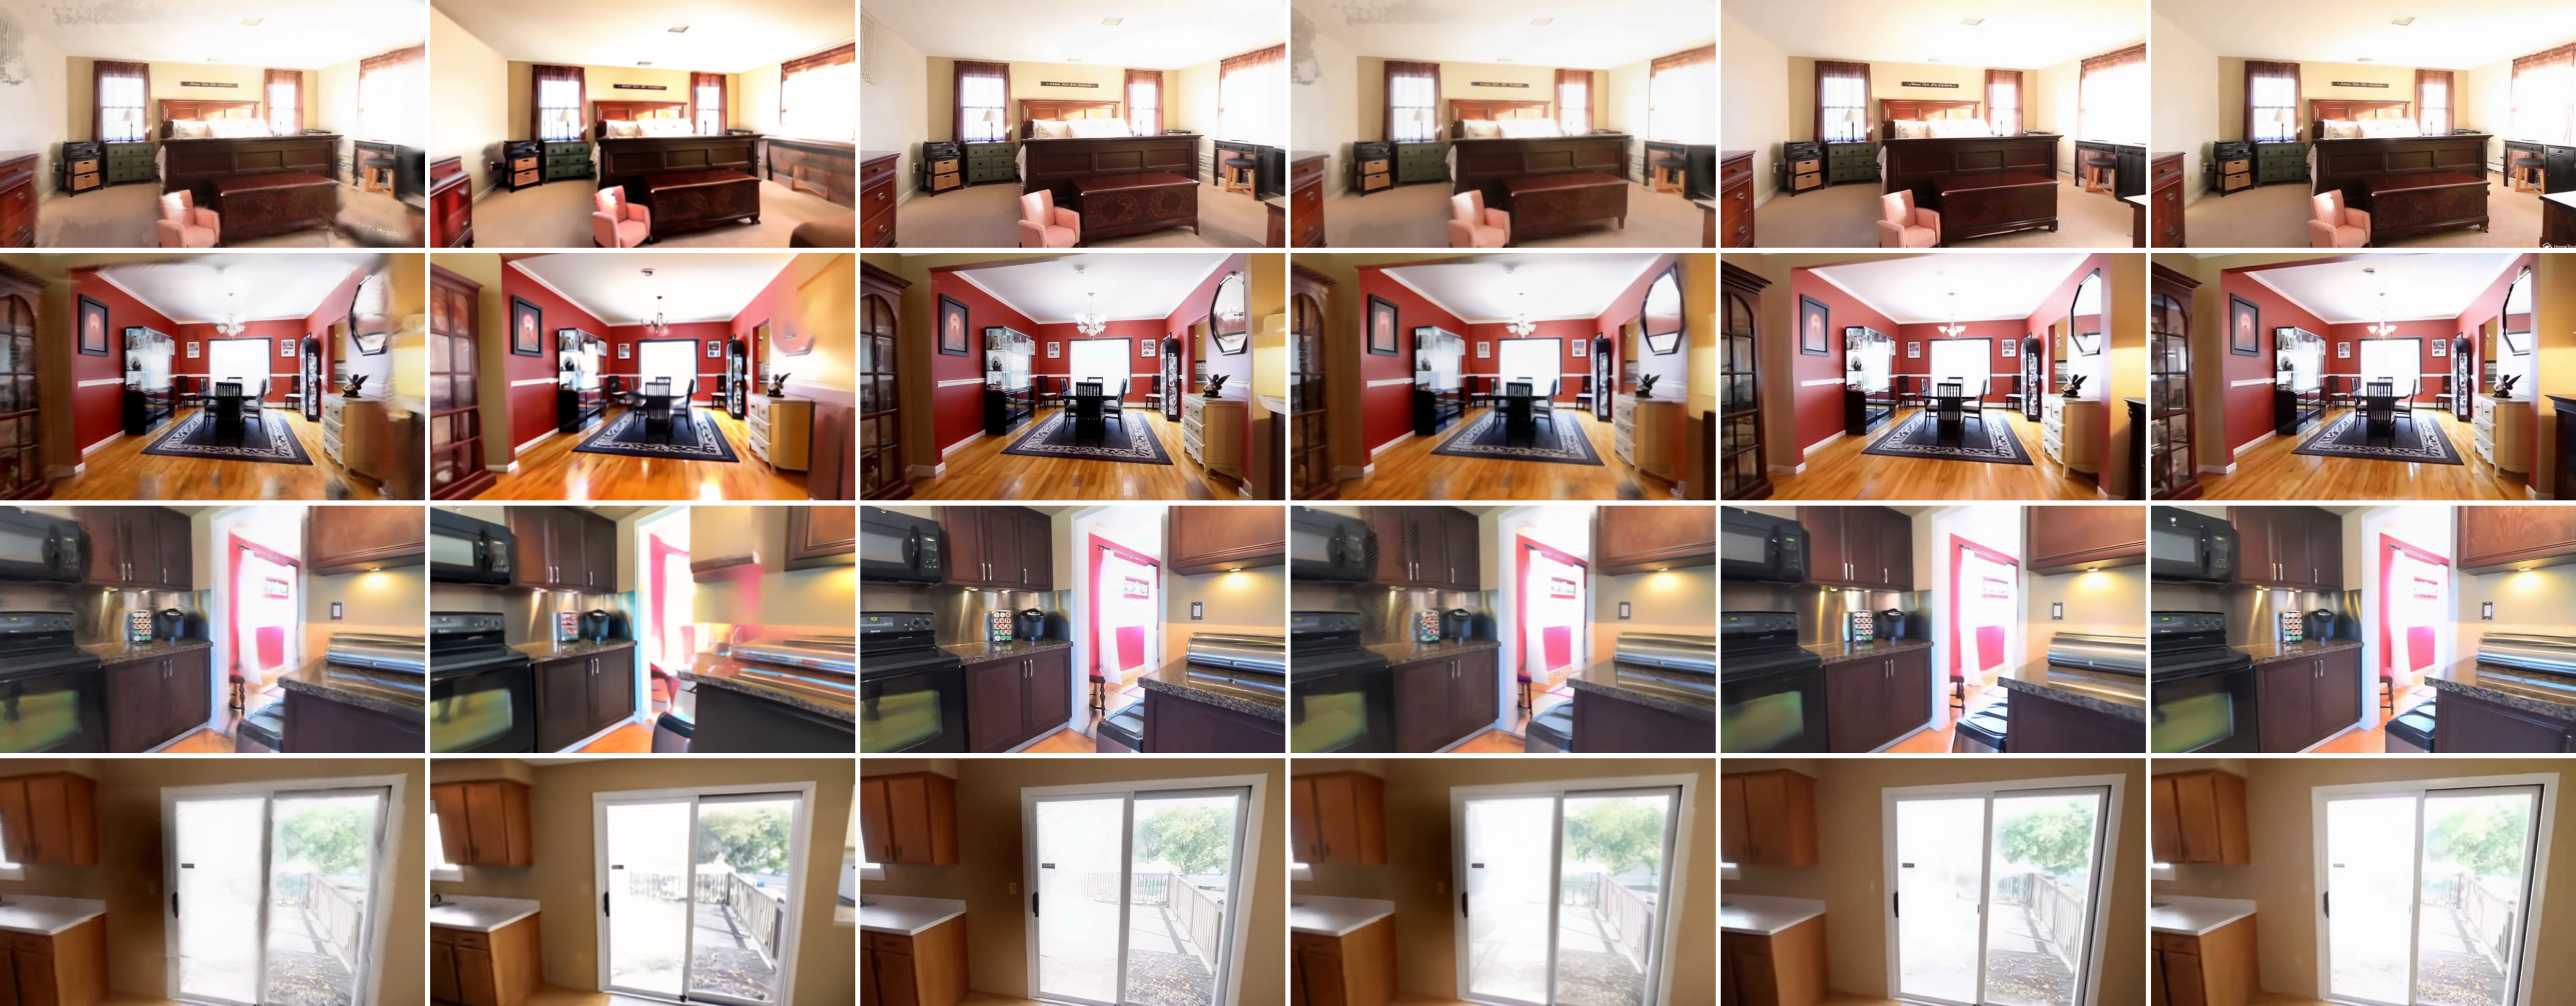
\includegraphics[width=\linewidth]{fig/image/supp_FF.png}%
    } \\
    \hspace{0.4cm} \small DepthSplat~\cite{xu2024depthsplat} & 
    \hspace{0.4cm} \small MVSplat360~\cite{chen2024mvsplat360} & 
    \hspace{.5cm}\small Difix3D+~\cite{wu2025difix3d} & 
    \hspace{.6cm}\small ExploreGS~\cite{Kim_2025_ExploreGS} &
    \hspace{0.2cm}\small \ours (Ours) & 
    \hspace{-0.1cm}\small Ground Truth \\

\end{tabular}  
   \caption{\textbf{Additional Qualitative Comparison on Novel-view Refinement on DL3DV~\cite{ling2024dl3dv} and RE10K~\cite{re10k}.} Top four rows showcase 3DGS optimization methods and bottom four rows feed-forward 3DGS methods as starting point of the refinement.
}

    \label{fig:supp_image_refine}
\end{figure*}





\begin{figure*}[t]
    \centering
    % 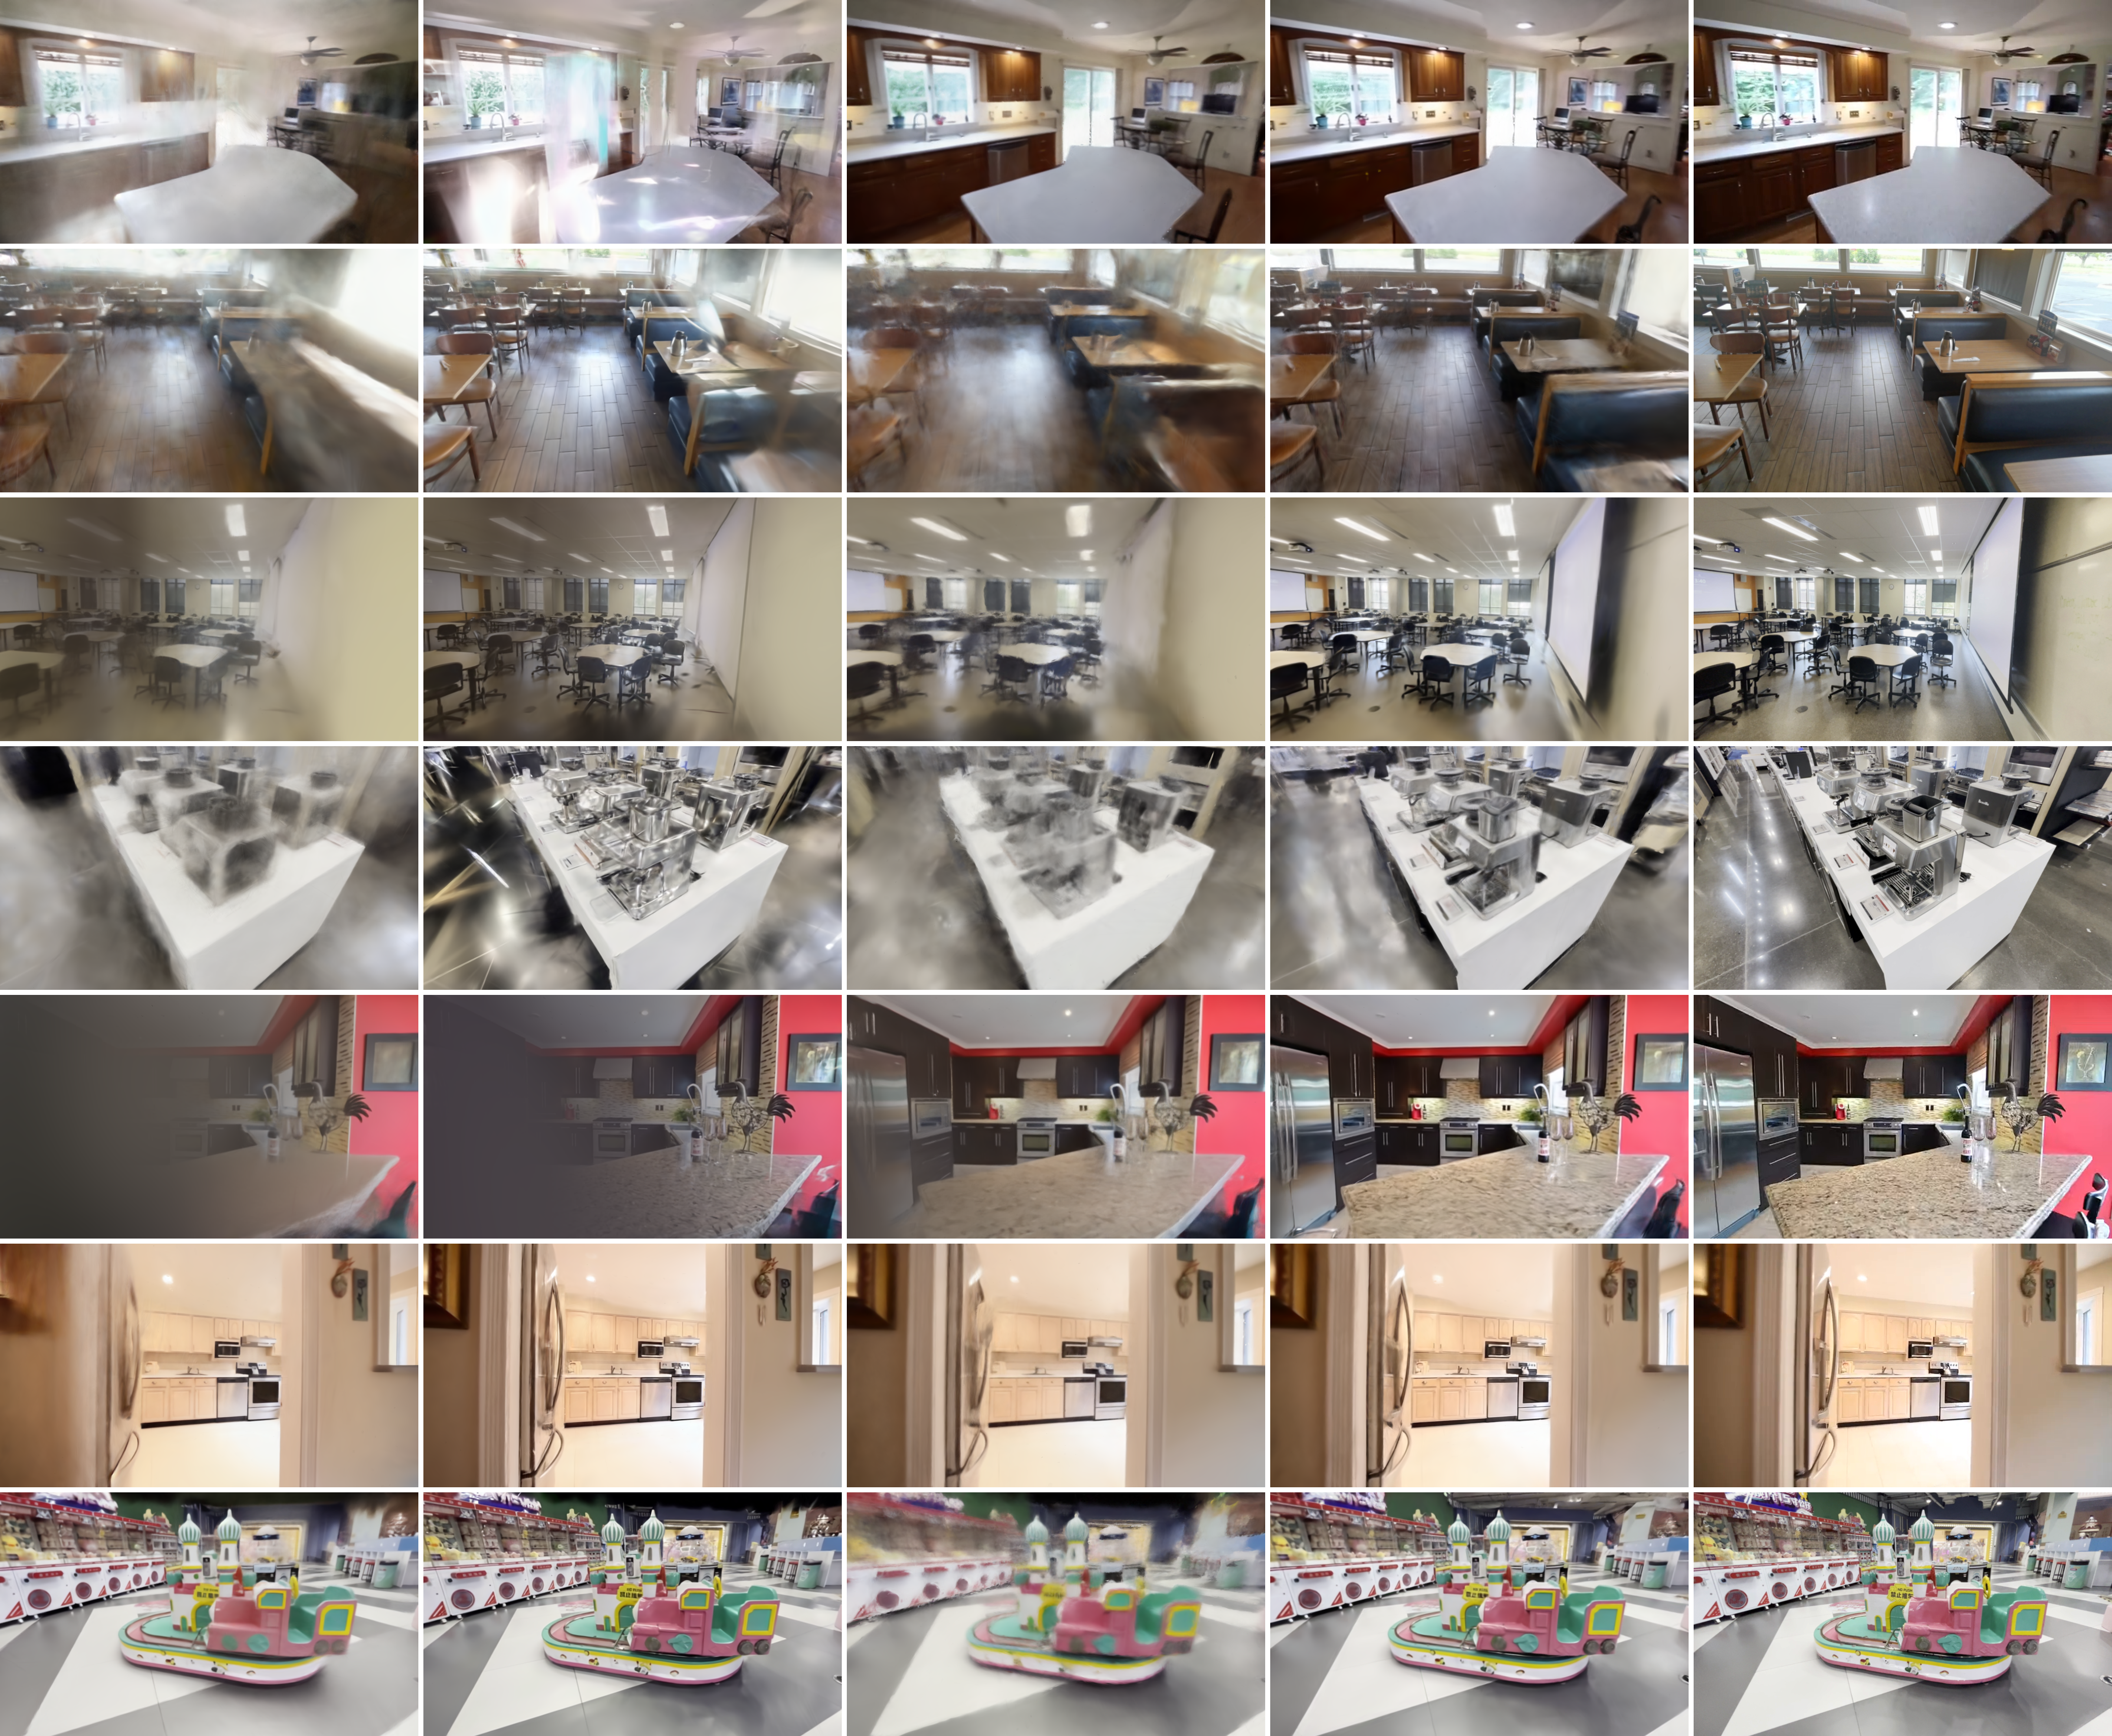
\includegraphics[width=\linewidth]{fig/image/supp_recon.png}
    
    \begin{tabular}{ccccc}
   
    \multicolumn{5}{c}{%
        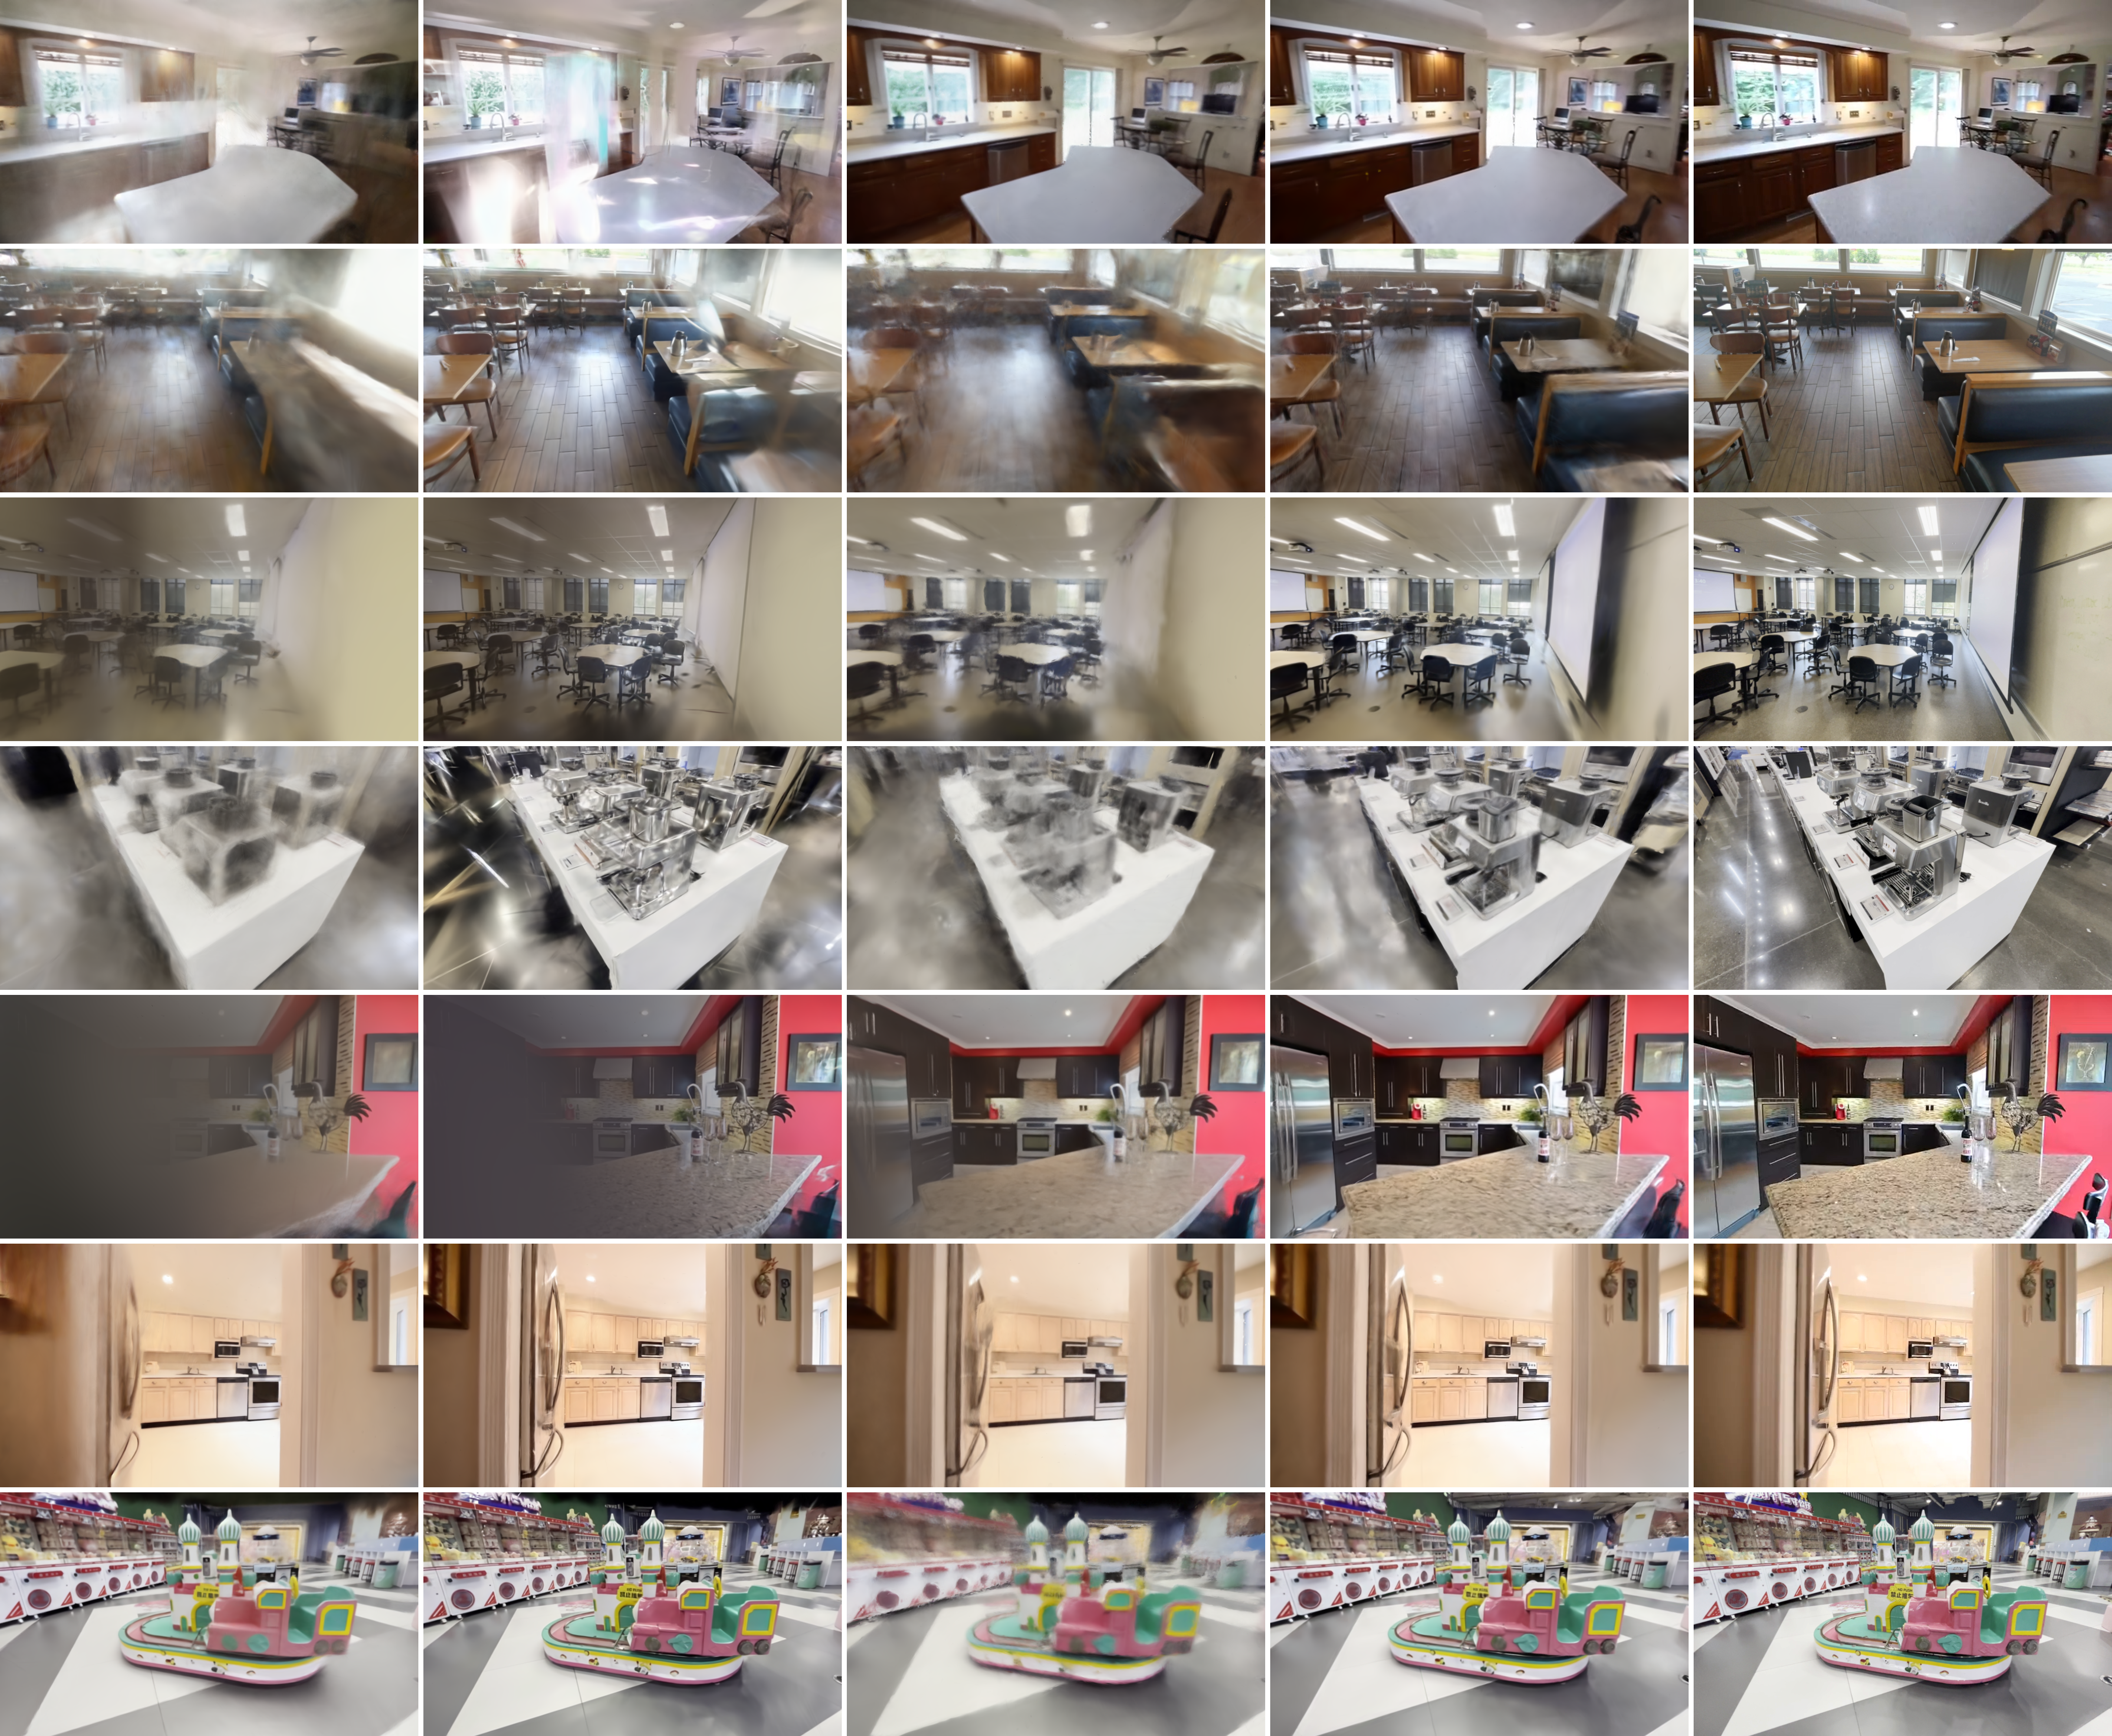
\includegraphics[width=\linewidth]{fig/image/supp_recon.png}%
    } \\
    \hspace{0.8cm} \small GenFusion~\cite{Wu2025GenFusion} & 
    \hspace{1.2cm}\small Difix3D+~\cite{wu2025difix3d} & 
    \hspace{1.2cm}\small ExploreGS~\cite{Kim_2025_ExploreGS} &
    \hspace{0.7cm}\small \ours (Ours) & 
    \hspace{-0.1cm}\small Ground Truth \\

\end{tabular}  
\caption{\textbf{Additional Qualitative Comparison on 3D Reconstruction on DL3DV~\cite{ling2024dl3dv} and RE10K~\cite{re10k}.} \ours showcases sharper and cleaner appearance and geometry compared to baseline methods.}
    \label{fig:supp_recon}
\end{figure*}


